\documentclass{beamer}
\usepackage{graphicx} % Required for inserting images
\title{The SYK Model and Non-Fermi Liquids}
\author{Jash Desai}
\institute{Brown University}
\date{May 3, 2024}


\begin{document}
\frame{\titlepage}

\begin{frame}{Fermi-Liquid Theory}

\begin{itemize}
    \item Originally posited by Landau in 60s. 
    \item Gave a pretty accurate description of a broad range of materials via the introduction of quasiparticles. 
    \item Theory built upon interacting Fermi gases and the use of Pauli exclusion principle to posit that momentum states may be re-normalized to reflect new values for important observables such as mass, etc.
    \item Important systems such as liquid $^{3}$He and most non-superconducting metals can be described by it.
\end{itemize}

\end{frame}

\begin{frame}{Non-Fermi Liquids}

\begin{itemize}
    \item We find that some recent system such as La$_{2-x}$Sr$_{x}$CuO$_{4}$ \cite{Takagi_1992}and BaFe$_{2}$(As$_{1-x}$P$_{x}$)$_{2}$\cite{Hayes_2016} have measuremetns that deviate from Fermi liquid theory. In particular, at low temperatures and low energy - the temperature to resistivity scaling.
    \begin{figure}
        \centering
        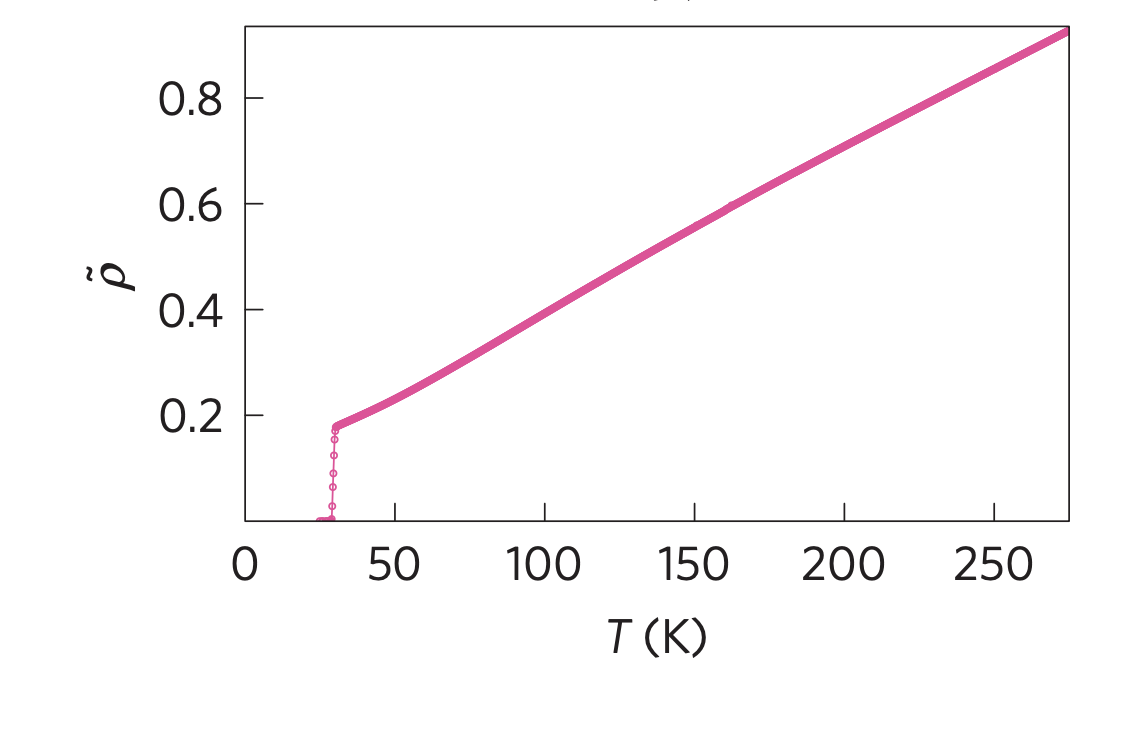
\includegraphics[scale = 0.4]{Linear.png}
        \caption{From \cite{Hayes_2016}. Measurement of BaFe$_{2}$(As$_{1-x}$P$_{x}$)$_{2}$ which deviates from Fermi liquid theory. }
        \label{fig:enter-label}
    \end{figure}
\end{itemize}
    
\end{frame}
\begin{frame}{Non-Fermi Liquids (cont.)}
\begin{itemize}
    \item Some other clues to Fermi-liquid theory breaking down are in strange metals and low energy symmetry breaking, measured in certain quantum spin liquids \cite{Tatsumi_2009}.
\end{itemize}
\begin{figure}
    \centering
    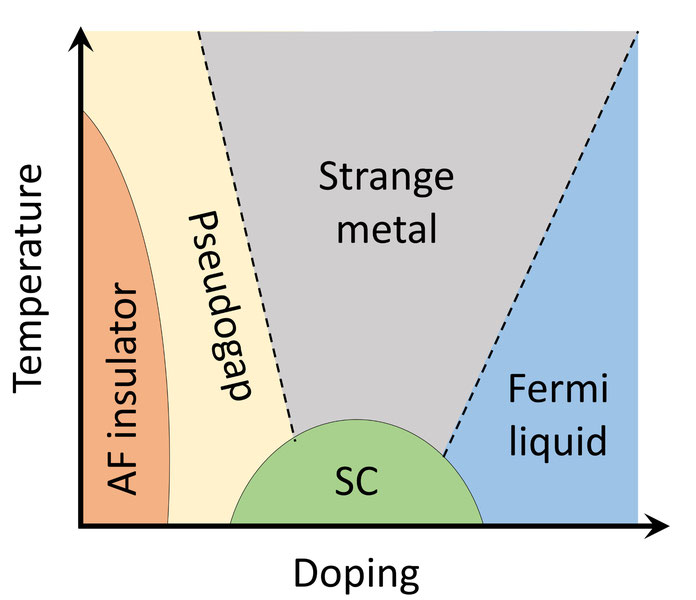
\includegraphics[scale = 0.2]{Strange Metal.jpeg}
    \caption{Informal strange metal diagram}
    \label{fig:enter-label}
\end{figure}
    
\end{frame}
\begin{frame}{Random Matrix Model}
\begin{itemize}
    \item So we have some clues to look for when considering alternative models. Let's take a look at the random matrix model first.
\end{itemize}
\begin{equation}
    H_{2} = \frac{1}{(N)^{1/2}}\sum_{i,j =1}^{N} t_{ij}c_{i}^{\dagger}c_{j} -  \mu \sum_{i}c_{i}^{\dagger}c_{i}
\end{equation}
\begin{itemize}
    \item Shows promise initially, but at closer look it just gets us back to a Fermi-liquid type explanation for exotic phenomenon. Quasiparticles are an indication of this.
\end{itemize}

\end{frame}
\begin{frame}{RMM (cont.)}
\begin{figure}
    \centering
    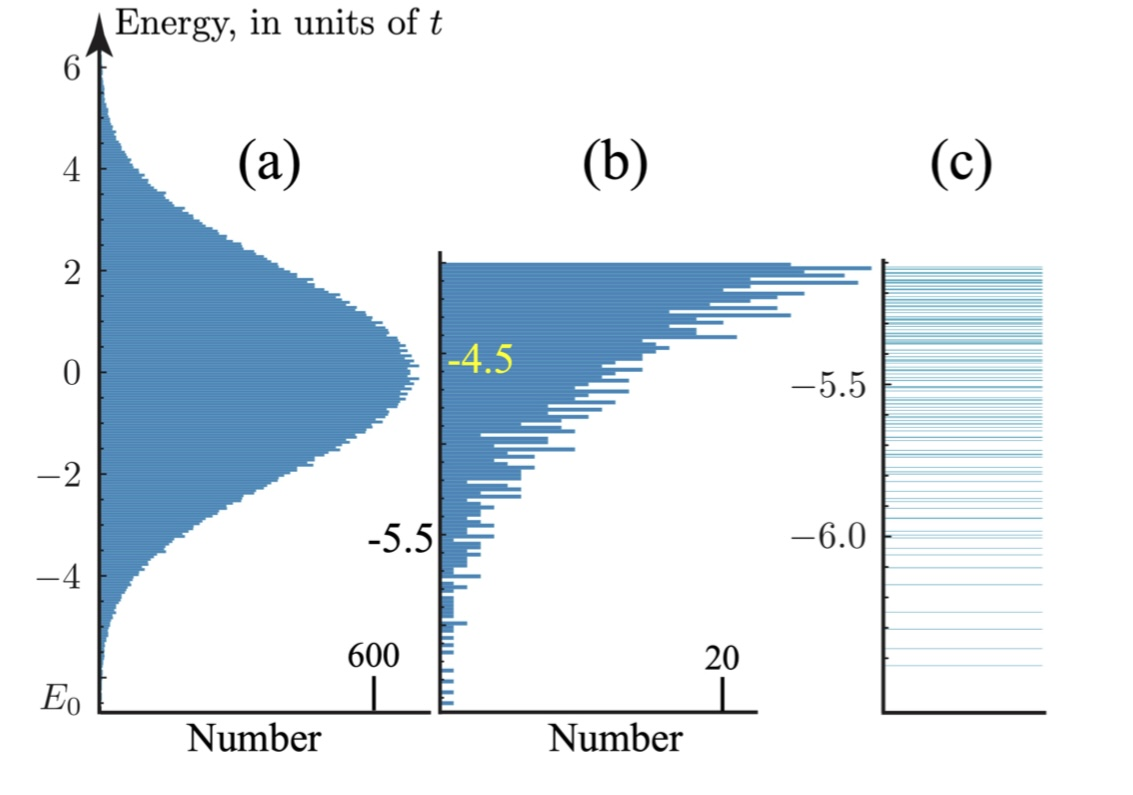
\includegraphics[scale = 0.4]{RandomMatrixSpectrum.jpeg}
    \caption{From \cite{Chowdhury_2022}, we have the many-body eigenvalues for N = 32 random matrix model. $\mathcal{N}$(E) is graphed out in (a) and (b) while (c) is the individual energy levels.}
    \label{fig:enter-label}
\end{figure}
    
\end{frame}
\begin{frame}{SYK Model}
\begin{equation}
    H_{4} = \frac{1}{(2N)^{3/2}} \sum_{ijkl =1}^{N} U_{ijkl} c_{i}^{\dagger}c_{j}^{\dagger}c_{k}c_{l} -  \mu \sum_{i}c_{i}^{\dagger}c_{i}
\end{equation}
\begin{itemize}
    \item This model looks more promising from the spectral analysis. It also does not have quasiparticles, meaning it is not constrained by the limitations of a model that would.
\end{itemize}
\end{frame}
\begin{frame}{SYK Model (cont.)}
\begin{figure}
    \centering
    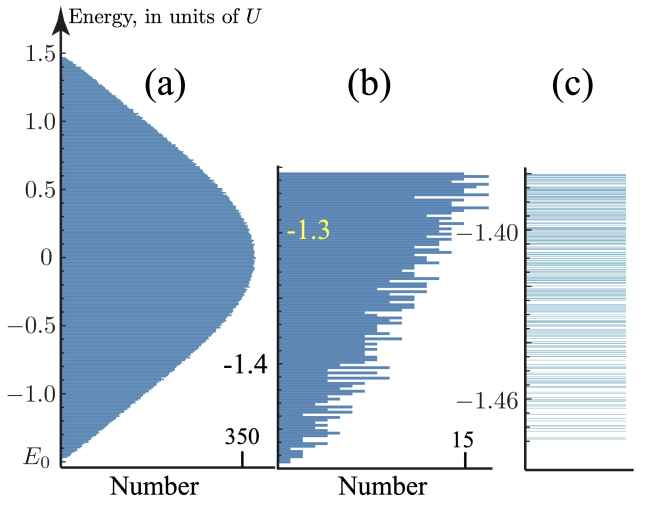
\includegraphics[scale = 0.6]{SYK Spectrum.png}
    \caption{From \cite{Chowdhury_2022}. The many-body eigenvalues of a $N$ = 32 Majorana SYK Hamiltonian. $\mathcal{N}$(E) is plotted in (a) and (b) while (c) shows the band energies.}
    \label{fig:enter-label}
\end{figure}
    
\end{frame}
\begin{frame}{Low Energy Limit of SYK}
\begin{itemize}
    \item Low energy limit immediately informs us model's utility via a numerical analysis.
    \item There are several iterations of the SYK model at low energies (e.g. SUSY versions, double-scaled version, etc.) but all of them maintain same key assumptions and same general structure of the Hamiltonian.
\end{itemize}
\begin{figure}
    \centering
    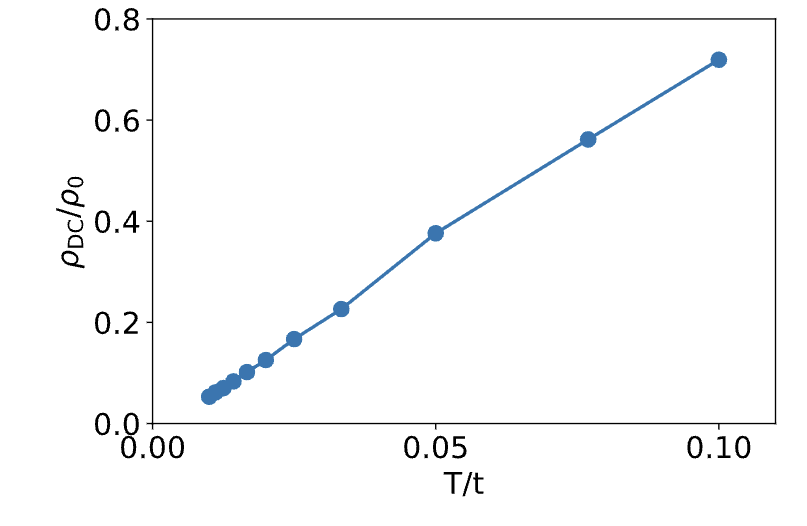
\includegraphics[scale = 0.4]{SYKLinear.png}
    \caption{From \cite{Cha_2020}. Resistivity $\rho_{DC}/\rho_{0}$ vs. temperature $T/t$ computed via analytic continuation of Green's function.}
    \label{fig:enter-label}
\end{figure}


\end{frame}
\begin{frame}{$N \rightarrow \infty$ Limit of SYK }
\begin{itemize}
    \item This is a more theoretical limit and lends itself to the holographic duality connection as well as the SYK model as a proxy for modeling black holes.
    \item However, it is also in this limit that a SYK lattice can be constructed such that it can be used as a solvable model of a strange metal.
    \begin{figure}
        \centering
        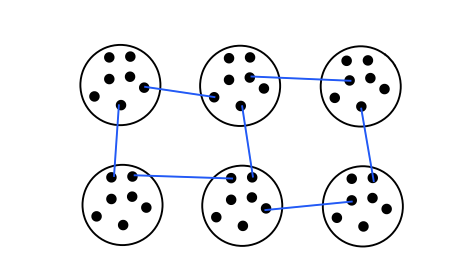
\includegraphics[scale = 0.8]{SYKLattice.png}
        \caption{Simple representation of the way a lattice may be constructed via the SYK model. The lattice is made up of SYK quantum dots with random interactions between dots.}
        \label{fig:enter-label}
    \end{figure}
\end{itemize}
\end{frame}
\begin{frame}{Conclusion}
    \begin{itemize}
        \item Fermi-liquid theory's use of quasiparticles hold it back from modeling several disordered and strongly correlated systems including non-Fermi liquids and strange metals.
        \item The random matrix model is able to reconstruct much of Fermi-liquid theory's range of interaction description without the explicit use of quasiparticles via random Fermionic couplings.
        \item The SYK model can go beyond the random matrix model with the use of random interactions and couplings with a quartic Majorana fermion model. The SYK model does not have quasiparticles.
        \item The low-energy limit of the SYK model recovers non-Fermi behavior such as linear resistivity.
        \item The high energy limit links the SYK model to black holes and thermofield calculations but also allows for the SYK model to be constucted as a working example of a strange metal.
    \end{itemize}

\end{frame}





\begin{frame}{Bibliography}
\bibliography{bibliography}
\bibliographystyle{abbrv}
    
\end{frame}
\end{document}

